% Options for packages loaded elsewhere
% Options for packages loaded elsewhere
\PassOptionsToPackage{unicode}{hyperref}
\PassOptionsToPackage{hyphens}{url}
%
\documentclass[
  english,
  russian,
  13pt,
  a4paper,
  DIV=11,
  numbers=noendperiod]{scrreprt}
\usepackage{xcolor}
\usepackage[left=3cm,right=1.5cm,top=2cm,bottom=2cm]{geometry}
\usepackage{amsmath,amssymb}
\setcounter{secnumdepth}{5}
\usepackage{iftex}
\ifPDFTeX
  \usepackage[T1]{fontenc}
  \usepackage[utf8]{inputenc}
  \usepackage{textcomp} % provide euro and other symbols
\else % if luatex or xetex
  \usepackage{unicode-math} % this also loads fontspec
  \defaultfontfeatures{Scale=MatchLowercase}
  \defaultfontfeatures[\rmfamily]{Ligatures=TeX,Scale=1}
\fi
\usepackage{lmodern}
\ifPDFTeX\else
  % xetex/luatex font selection
\fi
% Use upquote if available, for straight quotes in verbatim environments
\IfFileExists{upquote.sty}{\usepackage{upquote}}{}
\IfFileExists{microtype.sty}{% use microtype if available
  \usepackage[]{microtype}
  \UseMicrotypeSet[protrusion]{basicmath} % disable protrusion for tt fonts
}{}
\usepackage{setspace}
% Make \paragraph and \subparagraph free-standing
\makeatletter
\ifx\paragraph\undefined\else
  \let\oldparagraph\paragraph
  \renewcommand{\paragraph}{
    \@ifstar
      \xxxParagraphStar
      \xxxParagraphNoStar
  }
  \newcommand{\xxxParagraphStar}[1]{\oldparagraph*{#1}\mbox{}}
  \newcommand{\xxxParagraphNoStar}[1]{\oldparagraph{#1}\mbox{}}
\fi
\ifx\subparagraph\undefined\else
  \let\oldsubparagraph\subparagraph
  \renewcommand{\subparagraph}{
    \@ifstar
      \xxxSubParagraphStar
      \xxxSubParagraphNoStar
  }
  \newcommand{\xxxSubParagraphStar}[1]{\oldsubparagraph*{#1}\mbox{}}
  \newcommand{\xxxSubParagraphNoStar}[1]{\oldsubparagraph{#1}\mbox{}}
\fi
\makeatother


\usepackage{longtable,booktabs,array}
\usepackage{calc} % for calculating minipage widths
% Correct order of tables after \paragraph or \subparagraph
\usepackage{etoolbox}
\makeatletter
\patchcmd\longtable{\par}{\if@noskipsec\mbox{}\fi\par}{}{}
\makeatother
% Allow footnotes in longtable head/foot
\IfFileExists{footnotehyper.sty}{\usepackage{footnotehyper}}{\usepackage{footnote}}
\makesavenoteenv{longtable}
\usepackage{graphicx}
\makeatletter
\newsavebox\pandoc@box
\newcommand*\pandocbounded[1]{% scales image to fit in text height/width
  \sbox\pandoc@box{#1}%
  \Gscale@div\@tempa{\textheight}{\dimexpr\ht\pandoc@box+\dp\pandoc@box\relax}%
  \Gscale@div\@tempb{\linewidth}{\wd\pandoc@box}%
  \ifdim\@tempb\p@<\@tempa\p@\let\@tempa\@tempb\fi% select the smaller of both
  \ifdim\@tempa\p@<\p@\scalebox{\@tempa}{\usebox\pandoc@box}%
  \else\usebox{\pandoc@box}%
  \fi%
}
% Set default figure placement to htbp
\def\fps@figure{htbp}
\makeatother



\ifLuaTeX
\usepackage[bidi=basic,provide=*]{babel}
\else
\usepackage[bidi=default,provide=*]{babel}
\fi
% get rid of language-specific shorthands (see #6817):
\let\LanguageShortHands\languageshorthands
\def\languageshorthands#1{}


\setlength{\emergencystretch}{3em} % prevent overfull lines

\providecommand{\tightlist}{%
  \setlength{\itemsep}{0pt}\setlength{\parskip}{0pt}}



 
\usepackage[backend=biber,langhook=extras,autolang=other*]{biblatex}
\addbibresource{bib/cite.bib}

\usepackage[]{csquotes}

\KOMAoption{captions}{tableheading}
\usepackage{indentfirst}
\usepackage{float}
\floatplacement{figure}{H}
\usepackage{libertine}
\makeatletter
\@ifpackageloaded{caption}{}{\usepackage{caption}}
\AtBeginDocument{%
\ifdefined\contentsname
  \renewcommand*\contentsname{Содержание}
\else
  \newcommand\contentsname{Содержание}
\fi
\ifdefined\listfigurename
  \renewcommand*\listfigurename{Список иллюстраций}
\else
  \newcommand\listfigurename{Список иллюстраций}
\fi
\ifdefined\listtablename
  \renewcommand*\listtablename{Список таблиц}
\else
  \newcommand\listtablename{Список таблиц}
\fi
\ifdefined\figurename
  \renewcommand*\figurename{Рисунок}
\else
  \newcommand\figurename{Рисунок}
\fi
\ifdefined\tablename
  \renewcommand*\tablename{Таблица}
\else
  \newcommand\tablename{Таблица}
\fi
}
\@ifpackageloaded{float}{}{\usepackage{float}}
\floatstyle{ruled}
\@ifundefined{c@chapter}{\newfloat{codelisting}{h}{lop}}{\newfloat{codelisting}{h}{lop}[chapter]}
\floatname{codelisting}{Список}
\newcommand*\listoflistings{\listof{codelisting}{Листинги}}
\makeatother
\makeatletter
\makeatother
\makeatletter
\@ifpackageloaded{caption}{}{\usepackage{caption}}
\@ifpackageloaded{subcaption}{}{\usepackage{subcaption}}
\makeatother
\usepackage{bookmark}
\IfFileExists{xurl.sty}{\usepackage{xurl}}{} % add URL line breaks if available
\urlstyle{same}
\hypersetup{
  pdftitle={Лабораторная работа №4},
  pdfauthor={{[}Галиев Самир Салаватович{]}},
  pdflang={ru-RU},
  hidelinks,
  pdfcreator={LaTeX via pandoc}}


\title{Лабораторная работа №4}
\author{{[}Галиев Самир Салаватович{]}}
\date{Invalid Date}
\begin{document}
\maketitle

\renewcommand*\contentsname{Содержание}
{
\setcounter{tocdepth}{1}
\tableofcontents
}
\listoffigures
\listoftables

\setstretch{1.5}
\chapter{Лабораторная работа №4. Создание и процесс обработки программ
на языке ассемблера
NASM}\label{ux43bux430ux431ux43eux440ux430ux442ux43eux440ux43dux430ux44f-ux440ux430ux431ux43eux442ux430-4.-ux441ux43eux437ux434ux430ux43dux438ux435-ux438-ux43fux440ux43eux446ux435ux441ux441-ux43eux431ux440ux430ux431ux43eux442ux43aux438-ux43fux440ux43eux433ux440ux430ux43cux43c-ux43dux430-ux44fux437ux44bux43aux435-ux430ux441ux441ux435ux43cux431ux43bux435ux440ux430-nasm}

\textbf{Выполнил:} {[}Галиев Самир Салаватович{]}\\
\textbf{Группа:} {[}НКАбд-02-25{]}\\
\textbf{Дата выполнения:} {[}25.10.2025{]}

\section{Цель
работы}\label{ux446ux435ux43bux44c-ux440ux430ux431ux43eux442ux44b}

Освоение процедуры компиляции и сборки программ, написанных на
ассемблере NASM.

\section{Результаты выполнения лабораторной
работы}\label{ux440ux435ux437ux443ux43bux44cux442ux430ux442ux44b-ux432ux44bux43fux43eux43bux43dux435ux43dux438ux44f-ux43bux430ux431ux43eux440ux430ux442ux43eux440ux43dux43eux439-ux440ux430ux431ux43eux442ux44b}

\subsection{Описание выполняемого
задания}\label{ux43eux43fux438ux441ux430ux43dux438ux435-ux432ux44bux43fux43eux43bux43dux44fux435ux43cux43eux433ux43e-ux437ux430ux434ux430ux43dux438ux44f}

В ходе лабораторной работы необходимо было: 1. Создать простую программу
на языке ассемблера NASM, выводящую на экран сообщение \enquote{Hello
world!} 2. Освоить процесс трансляции исходного кода с помощью NASM 3.
Освоить процесс компоновки объектного файла с помощью LD 4. Запустить и
проверить работу исполняемого файла

\subsection{Скриншоты выполнения
заданий}\label{ux441ux43aux440ux438ux43dux448ux43eux442ux44b-ux432ux44bux43fux43eux43bux43dux435ux43dux438ux44f-ux437ux430ux434ux430ux43dux438ux439}

\subsubsection{Шаг 1: Создание рабочего
каталога}\label{ux448ux430ux433-1-ux441ux43eux437ux434ux430ux43dux438ux435-ux440ux430ux431ux43eux447ux435ux433ux43e-ux43aux430ux442ux430ux43bux43eux433ux430}

\begin{figure}[H]

{\centering \pandocbounded{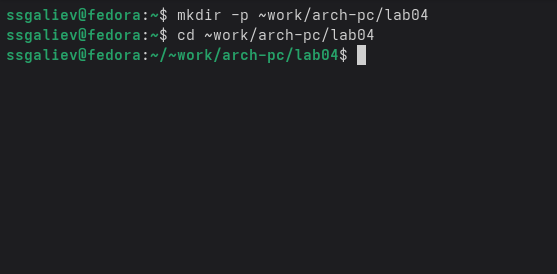
\includegraphics[keepaspectratio]{images/step1.png}}

}

\caption{Создание каталога lab04}

\end{figure}%

\subsubsection{Шаг 2: Создание и редактирование
hello.asm}\label{ux448ux430ux433-2-ux441ux43eux437ux434ux430ux43dux438ux435-ux438-ux440ux435ux434ux430ux43aux442ux438ux440ux43eux432ux430ux43dux438ux435-hello.asm}

\begin{figure}[H]

{\centering \pandocbounded{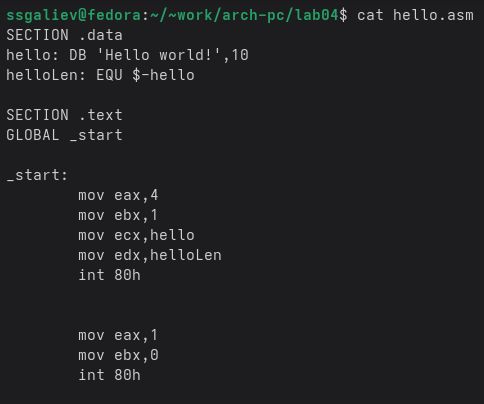
\includegraphics[keepaspectratio]{images/step2.png}}

}

\caption{Создание hello.asm}

\end{figure}%

\subsubsection{Шаг 3: Трансляция программы
NASM}\label{ux448ux430ux433-3-ux442ux440ux430ux43dux441ux43bux44fux446ux438ux44f-ux43fux440ux43eux433ux440ux430ux43cux43cux44b-nasm}

\begin{figure}[H]

{\centering \pandocbounded{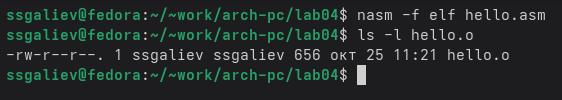
\includegraphics[keepaspectratio]{images/step3.png}}

}

\caption{Трансляция NASM}

\end{figure}%

\subsubsection{Шаг 4: Компоновка с помощью
LD}\label{ux448ux430ux433-4-ux43aux43eux43cux43fux43eux43dux43eux432ux43aux430-ux441-ux43fux43eux43cux43eux449ux44cux44e-ld}

\begin{figure}[H]

{\centering \pandocbounded{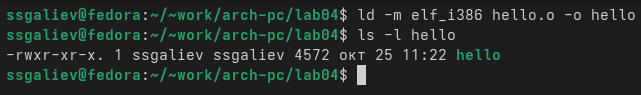
\includegraphics[keepaspectratio]{images/step4.png}}

}

\caption{Компоновка LD}

\end{figure}%

\subsubsection{Шаг 5: Запуск программы Hello
World}\label{ux448ux430ux433-5-ux437ux430ux43fux443ux441ux43a-ux43fux440ux43eux433ux440ux430ux43cux43cux44b-hello-world}

\begin{figure}[H]

{\centering \pandocbounded{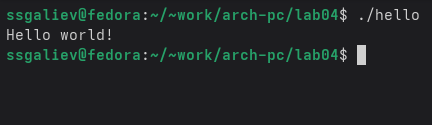
\includegraphics[keepaspectratio]{images/step5.png}}

}

\caption{Запуск программы}

\end{figure}%

\subsection{Комментарии и
выводы}\label{ux43aux43eux43cux43cux435ux43dux442ux430ux440ux438ux438-ux438-ux432ux44bux432ux43eux434ux44b}

В процессе выполнения основной части работы: 1. Успешно создана
программа на ассемблере NASM 2. Освоен процесс трансляции и компоновки
3. Программа выводит сообщение \enquote{Hello world!}

\section{Результаты выполнения заданий для самостоятельной
работы}\label{ux440ux435ux437ux443ux43bux44cux442ux430ux442ux44b-ux432ux44bux43fux43eux43bux43dux435ux43dux438ux44f-ux437ux430ux434ux430ux43dux438ux439-ux434ux43bux44f-ux441ux430ux43cux43eux441ux442ux43eux44fux442ux435ux43bux44cux43dux43eux439-ux440ux430ux431ux43eux442ux44b}

\subsection{Описание
задания}\label{ux43eux43fux438ux441ux430ux43dux438ux435-ux437ux430ux434ux430ux43dux438ux44f}

\begin{enumerate}
\def\labelenumi{\arabic{enumi}.}
\tightlist
\item
  Создать копию файла hello.asm с именем lab4.asm
\item
  Изменить программу для вывода фамилии и имени
\item
  Провести трансляцию, компоновку и запуск
\item
  Загрузить файлы на GitHub
\end{enumerate}

\subsection{Скриншоты
выполнения}\label{ux441ux43aux440ux438ux43dux448ux43eux442ux44b-ux432ux44bux43fux43eux43bux43dux435ux43dux438ux44f}

\subsubsection{Шаг 6: Создание lab4.asm и ее
запуск}\label{ux448ux430ux433-6-ux441ux43eux437ux434ux430ux43dux438ux435-lab4.asm-ux438-ux435ux435-ux437ux430ux43fux443ux441ux43a}

\begin{figure}[H]

{\centering \pandocbounded{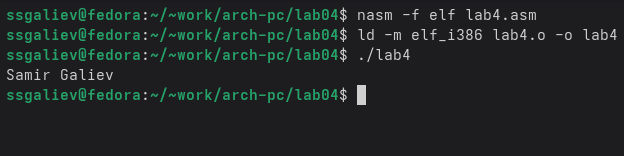
\includegraphics[keepaspectratio]{images/step6.png}}

}

\caption{Создание lab4.asm(запуск программы)}

\end{figure}%

\subsubsection{Шаг 7: Отредактированный hello.asm для
lab4.asm}\label{ux448ux430ux433-7-ux43eux442ux440ux435ux434ux430ux43aux442ux438ux440ux43eux432ux430ux43dux43dux44bux439-hello.asm-ux434ux43bux44f-lab4.asm}

\begin{figure}[H]

{\centering \pandocbounded{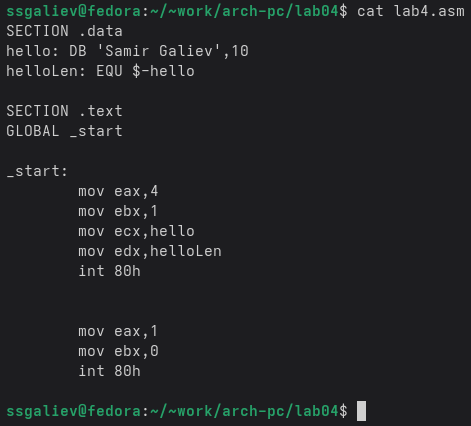
\includegraphics[keepaspectratio]{images/step7.png}}

}

\caption{Отредактированный hello.asm}

\end{figure}%

\subsubsection{Шаг 8: Загрузка на
GitHub}\label{ux448ux430ux433-8-ux437ux430ux433ux440ux443ux437ux43aux430-ux43dux430-github}

\pandocbounded{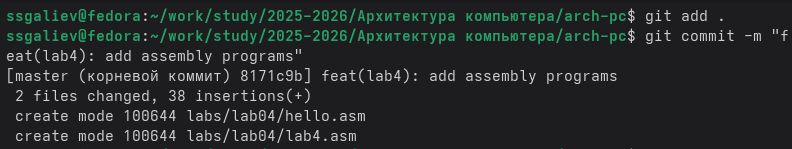
\includegraphics[keepaspectratio]{images/step9.png}}
\pandocbounded{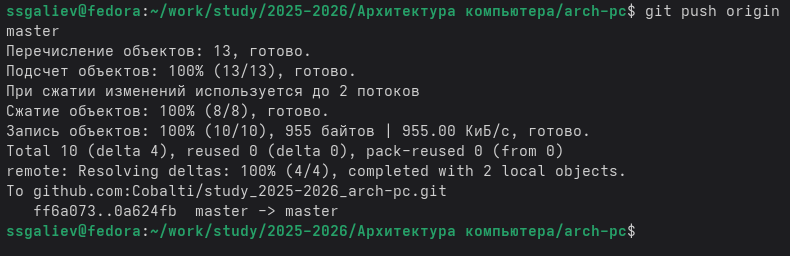
\includegraphics[keepaspectratio]{images/step10.png}}
\pandocbounded{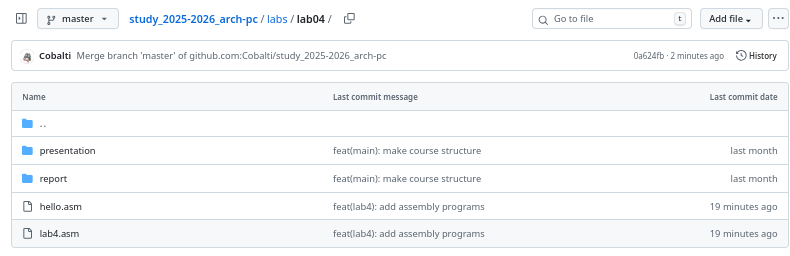
\includegraphics[keepaspectratio]{images/step11.png}}

\subsection{Листинги
программ}\label{ux43bux438ux441ux442ux438ux43dux433ux438-ux43fux440ux43eux433ux440ux430ux43cux43c}

\subsubsection{hello.asm}\label{hello.asm}

```nasm ; hello.asm SECTION .data hello: DB \enquote*{Hello world!},10
helloLen: EQU \$-hello

SECTION .text GLOBAL \_start

\_start: mov eax,4 mov ebx,1 mov ecx,hello mov edx,helloLen int 80h

\begin{verbatim}
mov eax,1
mov ebx,0
int 80h
\end{verbatim}

\subsection{Выводы}\label{ux432ux44bux432ux43eux434ux44b}

В ходе лабораторной работы была освоена процедура компиляции и сборки
программ на ассемблере NASM. Изучены этапы трансляции, компоновки и
запуска программ.

\subsection{Список
литературы}\label{ux441ux43fux438ux441ux43eux43a-ux43bux438ux442ux435ux440ux430ux442ux443ux440ux44b}

\begin{enumerate}
\def\labelenumi{\arabic{enumi}.}
\item
  \textbf{Официальная документация NASM}\\
  The NASM Documentation. --- URL: https://www.nasm.us/docs.php\\
  \emph{Официальная документация ассемблера NASM}
\item
  \textbf{Руководство по NASM на OpenNet}\\
  Расширенный ассемблер: NASM. --- URL:
  https://www.opennet.ru/docs/RUS/nasm/\\
  \emph{Подробное руководство на русском языке}
\item
  \textbf{Документация GNU LD}\\
  GNU LD Manual. --- URL: https://sourceware.org/binutils/docs/ld/\\
  \emph{Официальная документация компоновщика LD}
\item
  \textbf{Руководство по ассемблеру от ASMTutor}\\
  NASM Assembly Language Tutorials. --- URL: https://asmtutor.com/\\
  \emph{Практические уроки по программированию на NASM}
\item
  \textbf{Столяров А.В. - Программирование на NASM}\\
  Столяров А. Программирование на языке ассемблера NASM для OC Unix. ---
  2-е изд. --- М.: МАКС Пресс, 2011. --- URL:
  http://www.stolyarov.info/books/asm\_unix\\
  \emph{Учебное пособие по NASM для Unix-систем}
\end{enumerate}


\printbibliography



\end{document}
